\label{sec:ProtokolDesign}

\textbf{Message Header}

Eine zentrale Rolle bei der Entwicklung des Aufbaus und der Strukturierung
spielte der Nachrichtenheader.
Dieser beinhaltet Informationen, die zum eindeutigen Versenden und Identifizieren der
mitgelieferten Daten notwendig sind. Dazu gehören die Versionsnummer,
die Konfiguration, die Länge der Nachricht und die genauen Adressen
des Senders und Empfängers. Neben dem Header sind die verpackten Daten, der
sogenannte Payload, und ein CRC-Code zur Fehlerüberprüfung der Nachricht
vorhanden. In Abbildung \ref{fig:DatenaufschluesselungMessage} ist der Header
einer Nachricht im Detail dargestellt.

\begin{figure}[H]
	\centering
	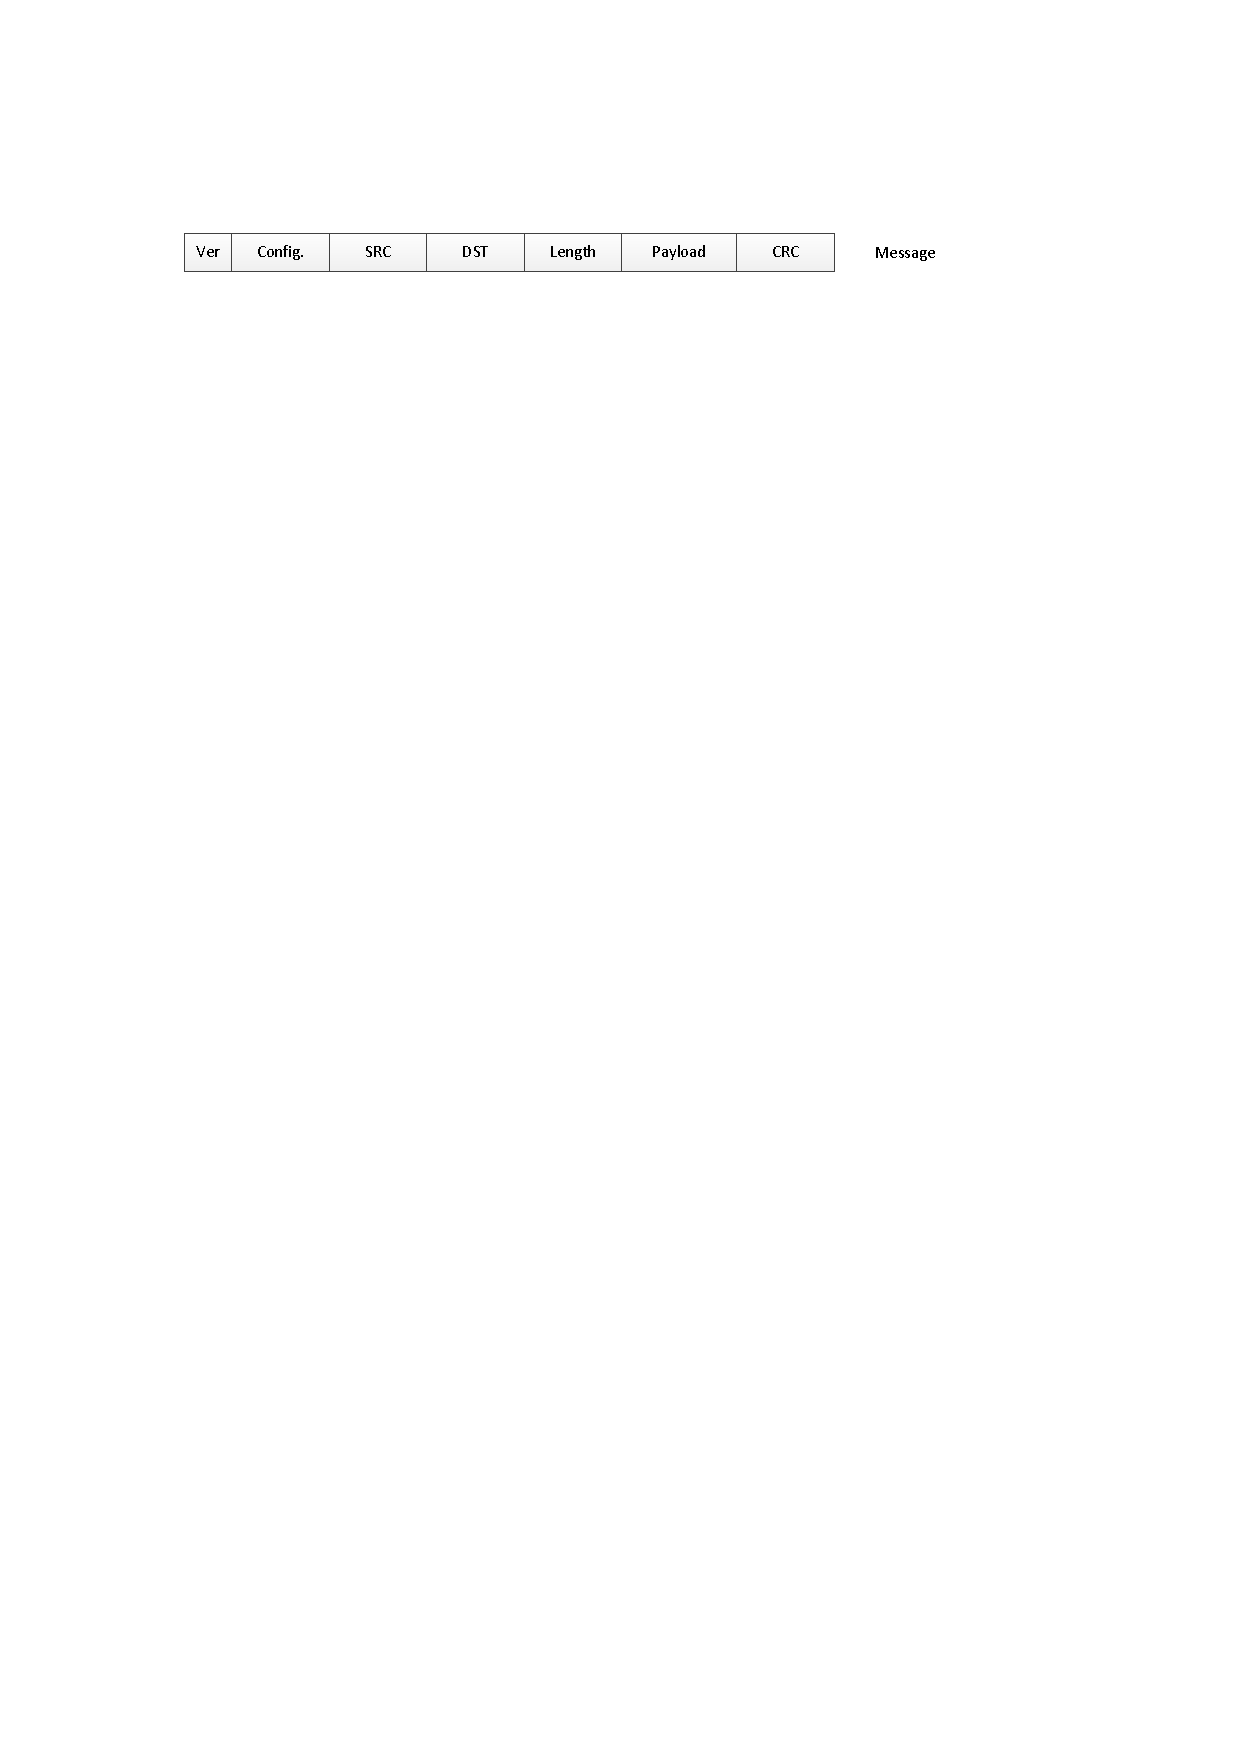
\includegraphics[width=\textwidth]{DatenaufschluesselungMessage.pdf}
	\caption{Datenaufschlüsselung der Nachricht}
	\label{fig:DatenaufschluesselungMessage}
\end{figure}

Die Versionsnummer belegt die ersten vier Bits des Headers. Diese
signalisiert dem Empfänger mit welcher Version des Protokolls die Nachricht
verpackt und versandt wurde. Danach folgt die Konfiguration. Mit Hilfe dieser,
können Einstellungen vorgenommen werden, welche die Größe der gesamten Nachricht
beeinflussen. Somit ist in speziellen Fällen eine bandbreitenschonende
Übertragung der Nachricht möglich, da keine ungenutzten Informationen oder Bits
vorhanden sind. Für die Konfiguration wurden $12$ Bits reserviert. Die ersten drei Bits
bestimmen das Adressformat. Dieses ermöglicht das Aufsetzen des Protokolls auf
bereits bestehenden Standards, wie IPv6 oder das Bundle-Protokoll.
Die verbleibenden neun Bits sind für zusätzliche Einstellungsmöglichkeiten zur Erweiterung des
Protokolls reserviert. Die Bitvergabe der Adressen von Sender und Empfänger
erfolgt dynamisch und in Abhängigkeit von der Konfiguration.
Dies ist für die Nutzung unterschiedlicher Übertragungsprotkolle notwendig.
Für IPv6 werden $256$ Bit bereitgestellt. Dies sind jeweils $128$ Bit für
die Sender- und Empfängeradresse. Die Länge repräsentiert die Größe der gesamten
Nachricht in Bytes und belegt die nächsten $24$ Bits.
Der vorletzte Bestandteil der Nachricht, der sogenannte Payload, beinhaltet die
eigentlichen Daten und besteht aus mehreren Datenblöcken. Zusätzlich werden am
Ende die Prüfsummenbits zur Fehlererkennung hinzugefügt. Diese sind $16$ Bits lang,
wenn die Gesamtlänge der Nachricht kleiner gleich $2^{16}$ Bytes ist.
Andernfalls beträgt die Länge $32$ Bits. Durch diese Unterteilung kann
Overhead vermieden werden wobei eine {\"U}bertragung gr{\"o}{\ss}erer
Nachrichten dennoch gew{\"a}rleistet bleibt.

\begin{figure}[H]
	\centering
	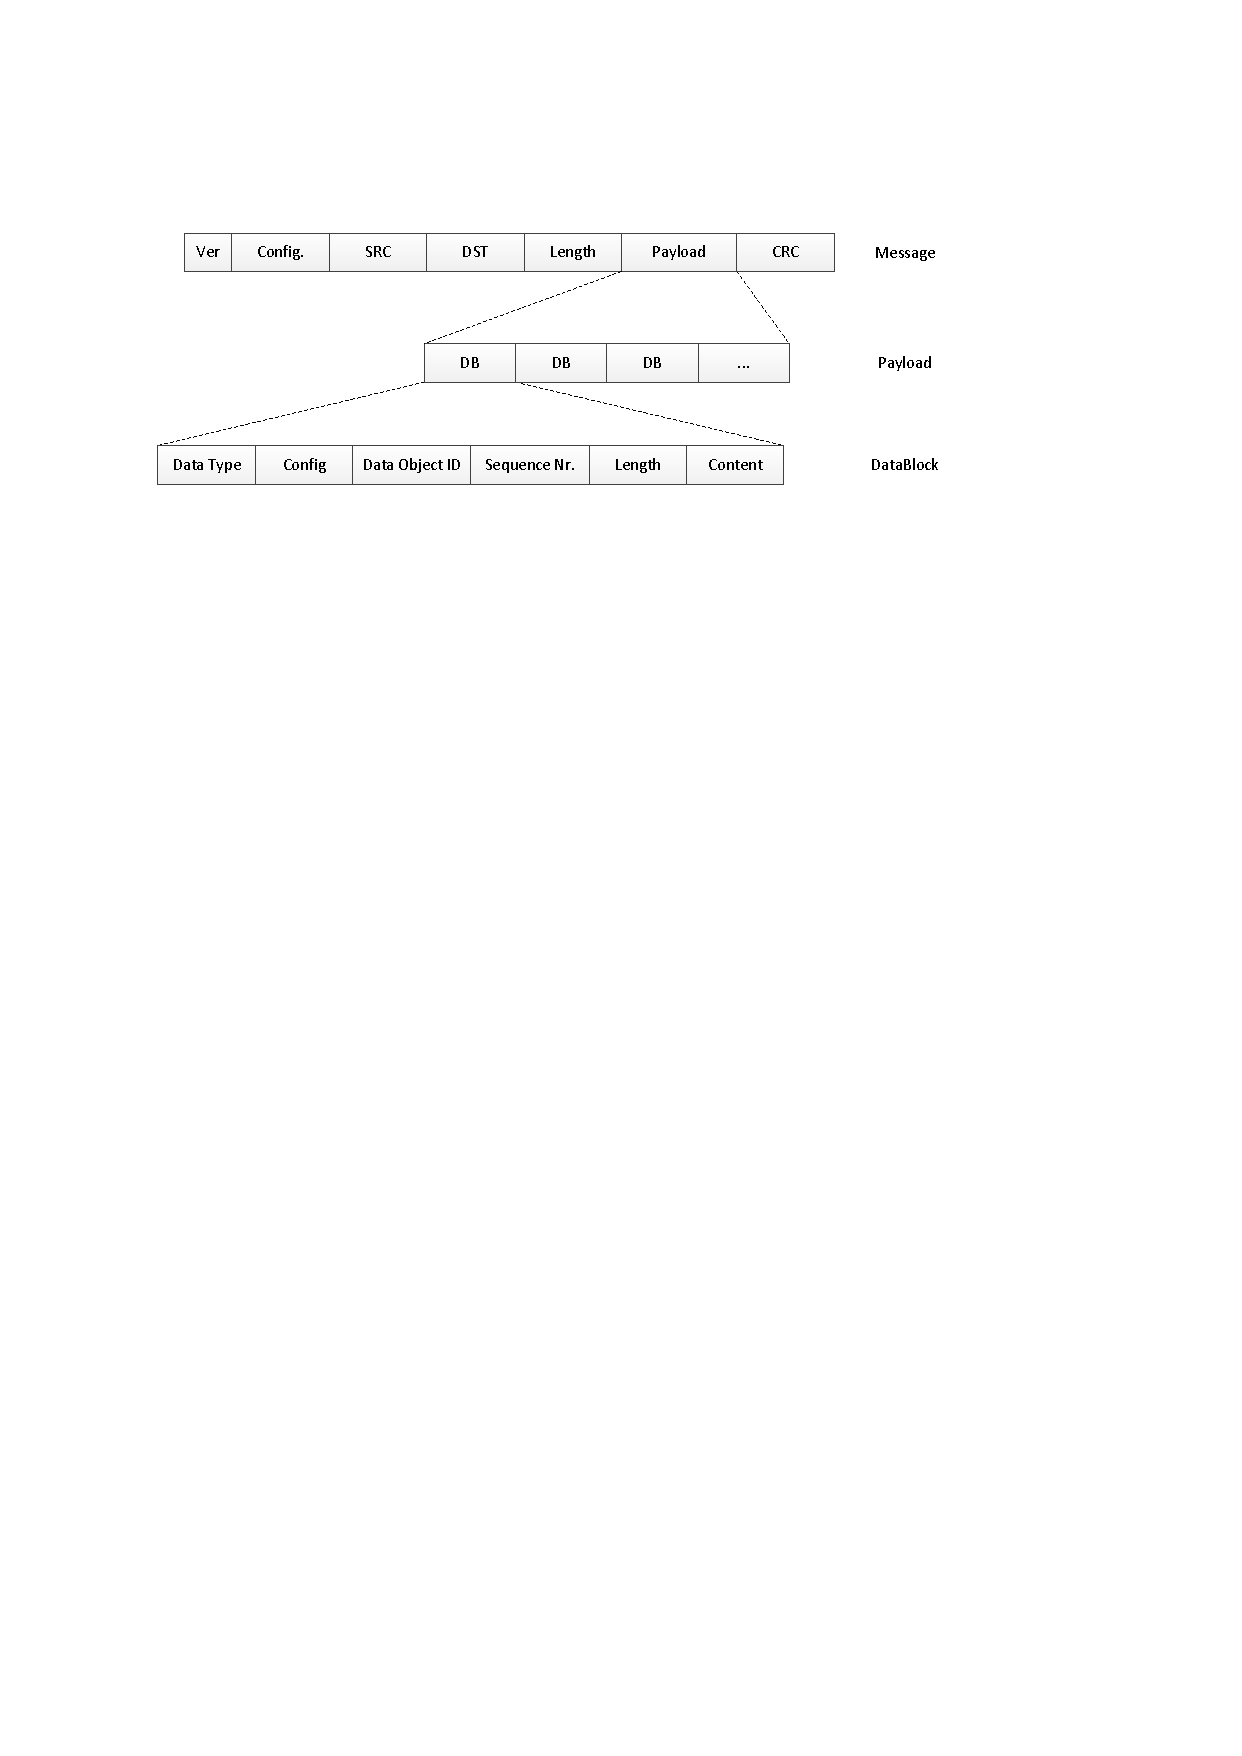
\includegraphics[width=\textwidth]{DatenaufschluesselungDB.pdf}
	\caption{Aufschlüsselung der Datenblöcke}
  \label{fig:DatenaufschluesselungDB}
\end{figure}

\textbf{Datenblockheader}

Eine schnelle und eindeutige Zuordnung eines einzelnen Datenblocks auf der
Empfängerseite, stand bei der Entwicklung des Headers im Mittelpunkt.
Dies bedeutet, dass neben der Bitvergabe eine genaue Überlegung über die
richtige Reihenfolge notwendig ist. Hierzu gibt es drei Ansätze, welche in
Abbildung \ref{fig:DatenblockVarianten} dargestellt sind.

\begin{figure}[H]
	\centering
	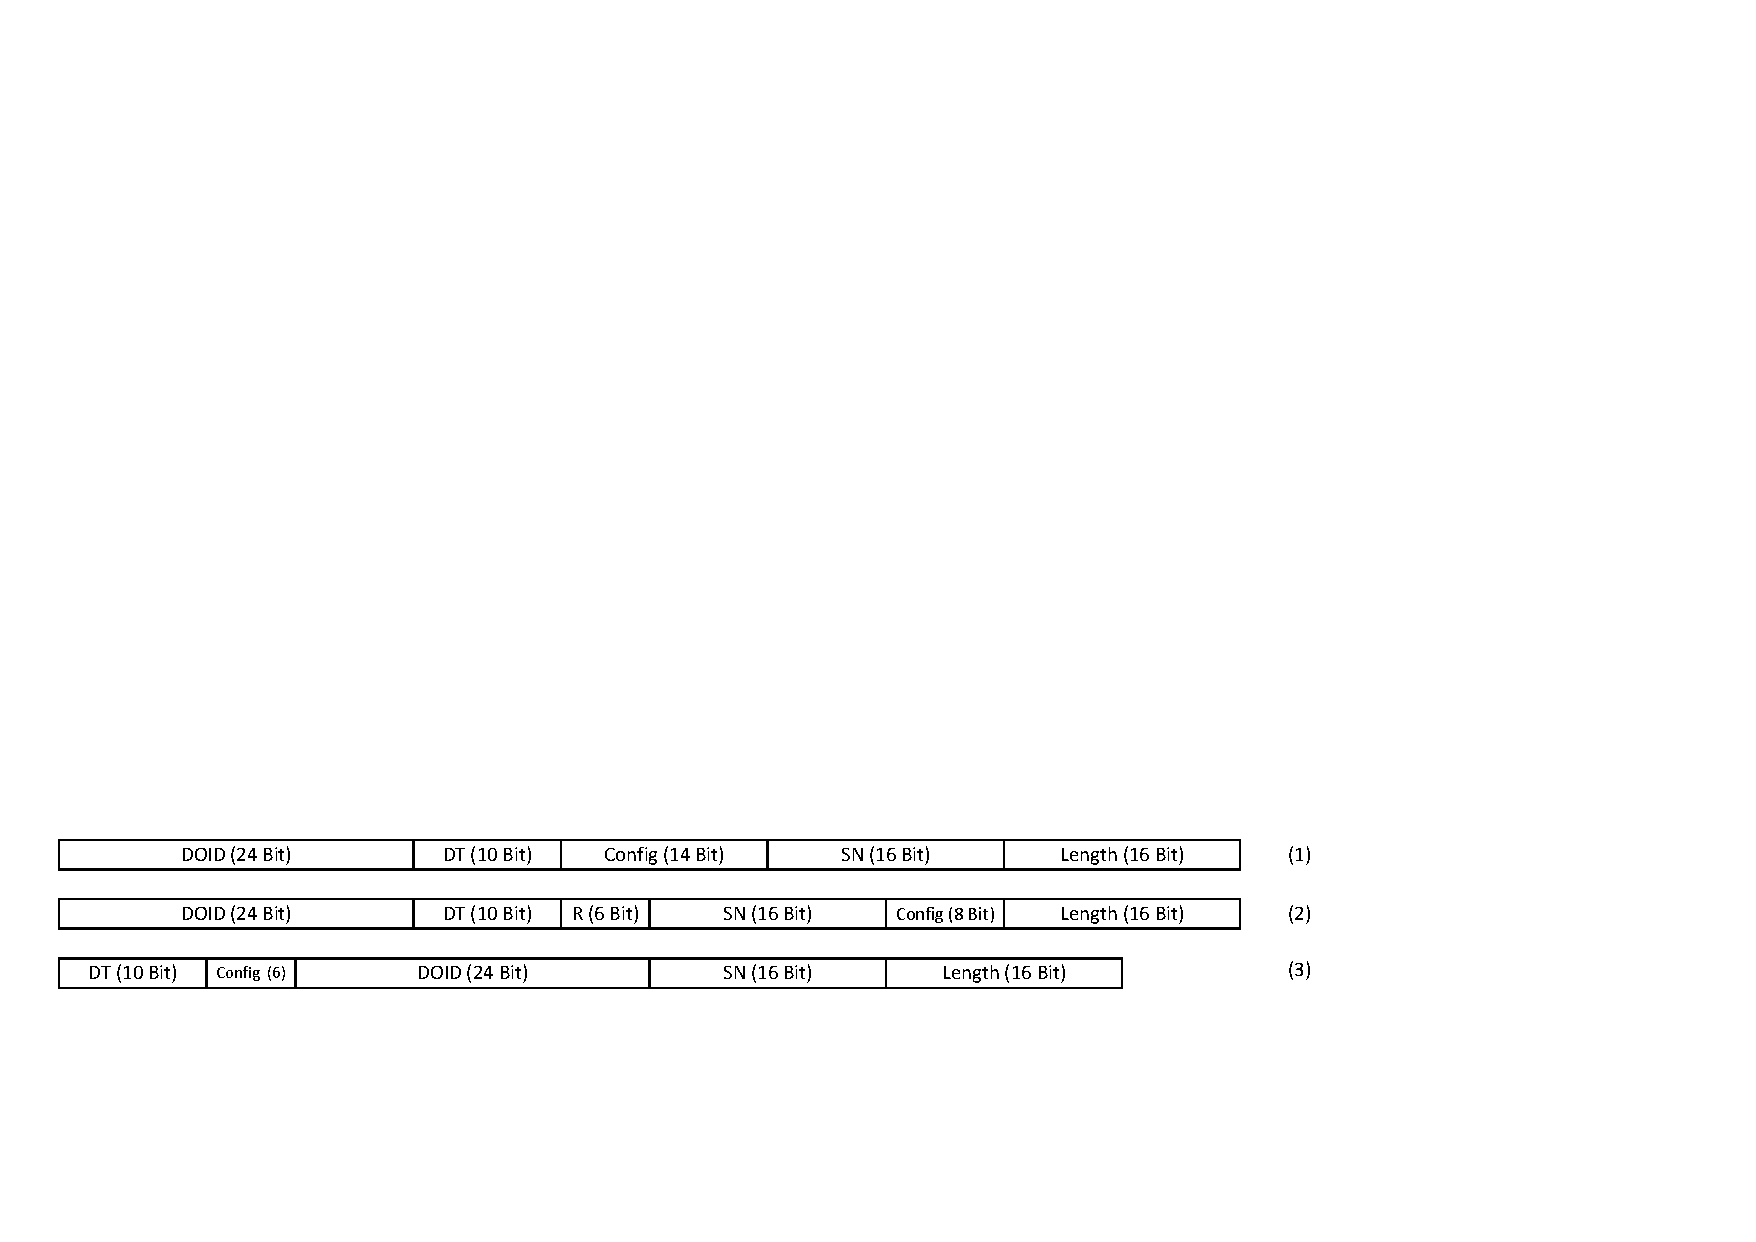
\includegraphics[width=\textwidth]{DatenblockVarianten.pdf}
	\caption{Ansätze des Datenblockheaders}
  \label{fig:DatenblockVarianten}
\end{figure}

Ein Datenblock besteht aus den folgenden Teilen: \gls{DOID}, Datentyp,
Konfiguration, Sequenznummer und der Länge des Datenblocks. Die \gls{DOID}
repräsentiert die Datei (Bild, Text, Sensorwerte,\etc) dem der Datenblock
angehört. Das Differenzieren der einzelnen Datenblöcke untereinander erfolgt
mittels der Sequenznummer. Durch die Einführung eines Datentyps im Header wird
der Bereich der \gls{DOID} indirekt vergrößert. Dies ist aufgrund der
eindeutigen Zuordnung einer \gls{DOID} zu einem Datentyp möglich.
\newline
Ausgegangen wurde anfangs von je acht Bit für den Datentyp und
die Konfiguration.
In diesem Zusammenhang wurde hinterfragt, ob die Bitvergabe ausreicht,
da sehr viele verschiedene Datentypen und Formate existieren. Infolgedessen
wurde, wie in Variante $1$ zu sehen, ein zusätzliches Byte zur Verfügung
gestellt. Dieses ist aufgeteilt in zwei Bit für den Datentyp und sechs Bit für
die Konfiguration. Die Idee hinter dieser Variante war, dass der Datenblock als
erstes über die \gls{DOID} und im Folgenden dem zugeordneten Datentyp identifiziert
wird. Anschließend sollten die Konfiguration und die Sequenznummer folgen.
Ein ähnlicher Aufbau gilt ebenfalls für Möglichkeit $2$, bei der die restlichen
sechs Bit zur Vorreservierung größerer Datentypen genutzt wurden. Dies war
bezüglich des Datentyps und der Menge unterschiedlicher Datenblöcke die bessere
Variante. Eine effektivere Maßnahme ergab sich am Ende nicht aus dem
Spendieren eines zusätzlichen Bytes, sondern aus einer anderen Reihenfolge in
der die Bestandteile im Header angeordnet sind. Wie in Variante $3$ ersichtlich,
wurden sechs Bit gespart. Dadurch wird zuerst jeder Datenblock anhand
seines Datentypes identifiziert und anschliessend durch die \gls{DOID} und die
Sequenznummer spezifiziert. Danach folgt die Konfiguration mit $6$ Bits.
Dabei sind die vordersten drei Bits die Kompression des Datenblockheaders, damit
kann die Länge der \gls{DOID}, der Sequenznummer und die Länge des gesamten
Datenblockes varrieren. Dadurch können auch kompakte Blöcke effizient
verschickt werden.
Das vierte Bit gibt an, ob ein Zeitstempel nach dem Header und vor einem
Datenpaket mit einer Länge von $8$ Byte gesetzt wird.
Dieses Bit wurde in der Konfiguration eingeführt, weil bei einigen Datentypen
nicht zwingend eine Zeitangabe benötigt wird und somit Overhead vermieden
werden kann. Für Daten mit konstanter aber geringer Größe können mehrere Werte
gleichzeitig in einem Datenblock platziert werden. Diese besitzen bei
gesetztem Zeitbit eine eigene Zeitangabe. Die Abbildung
\ref{fig:uebersichtdatenaufschluesselung} stellt diese Sachverhalte noch einmal
übersichtlich dar, diese werden im Anhang \ref{sec:messtabellen} noch
einmal in einer geb{\"u}hrenden Ausführung dargestellt.

\begin{figure}[H]
  \centering
  \subfigure[Sensor]{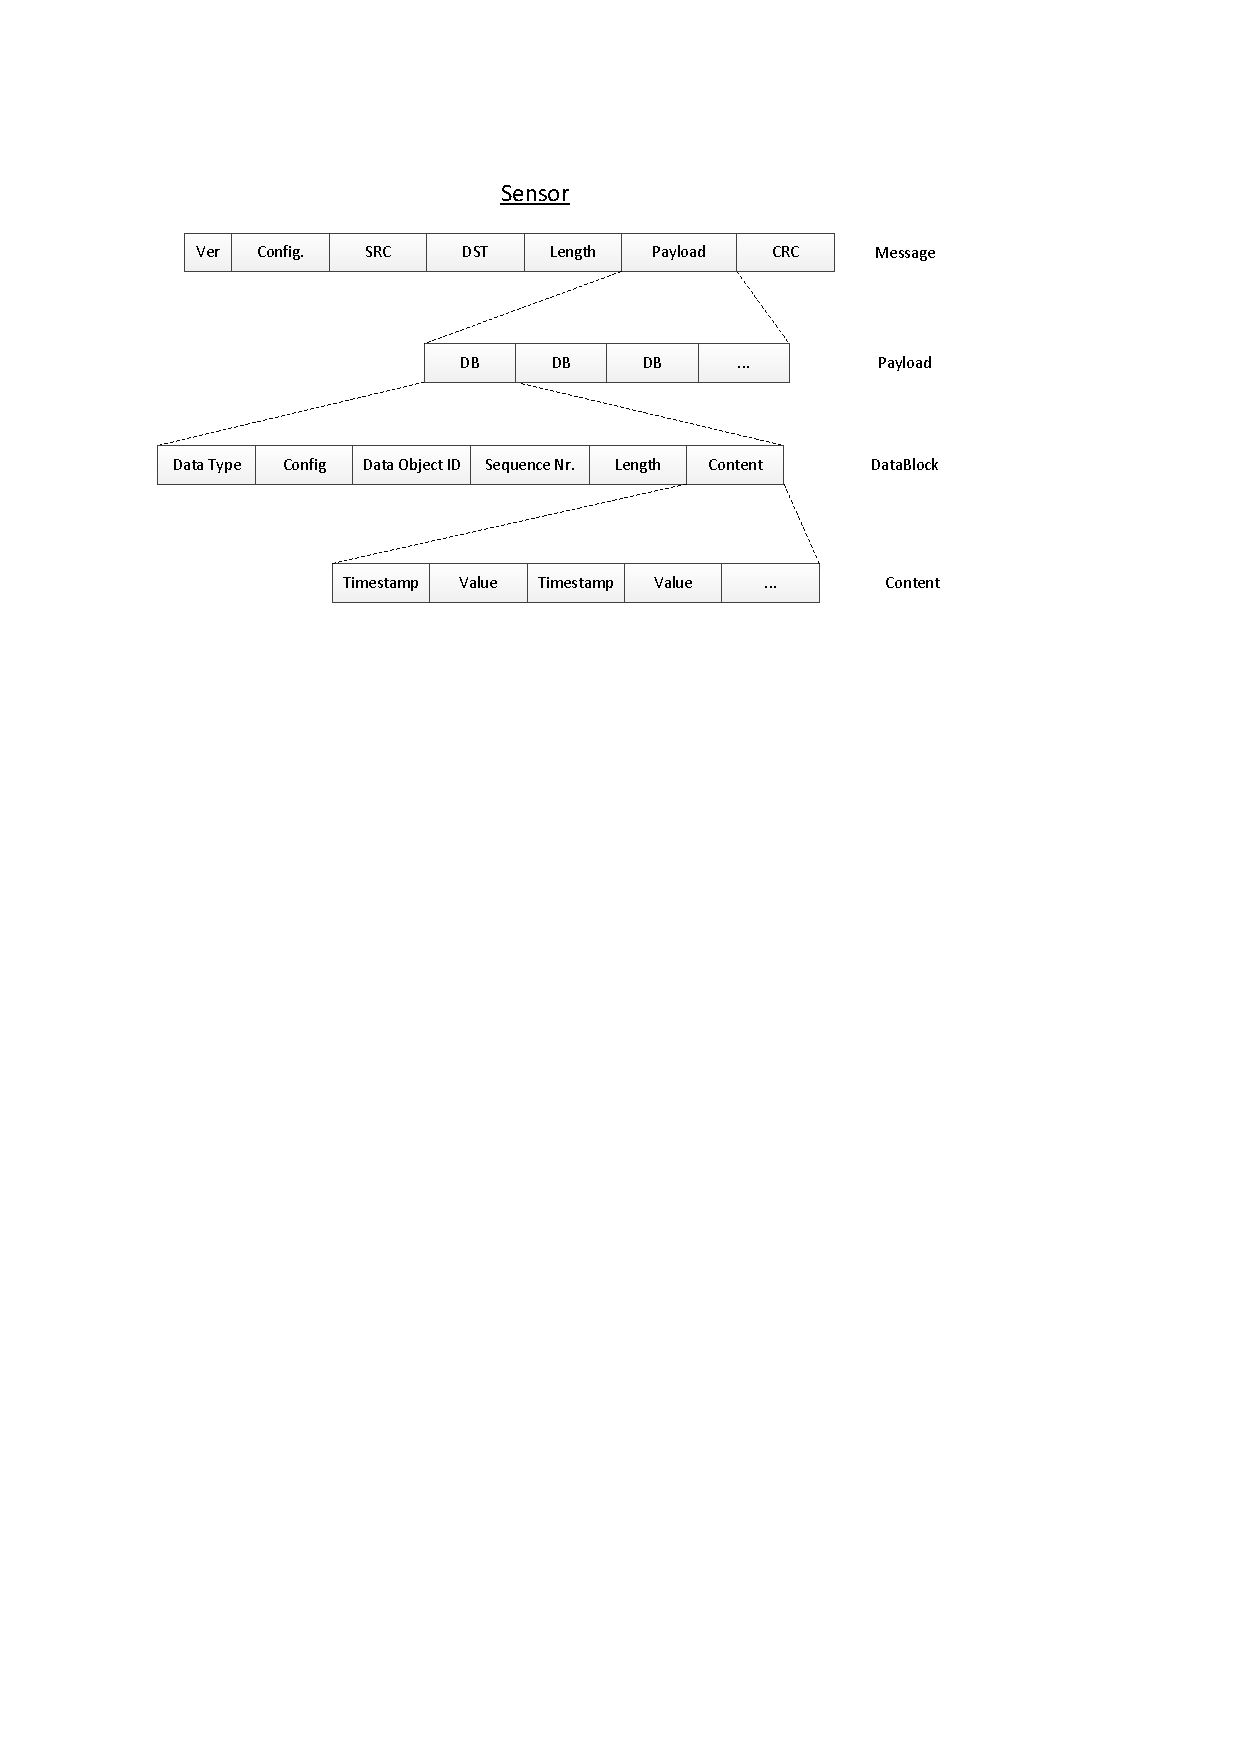
\includegraphics[width=\textwidth/2]{DatenaufschluesselungSensor.pdf}}\hfill
  \subfigure[Text]{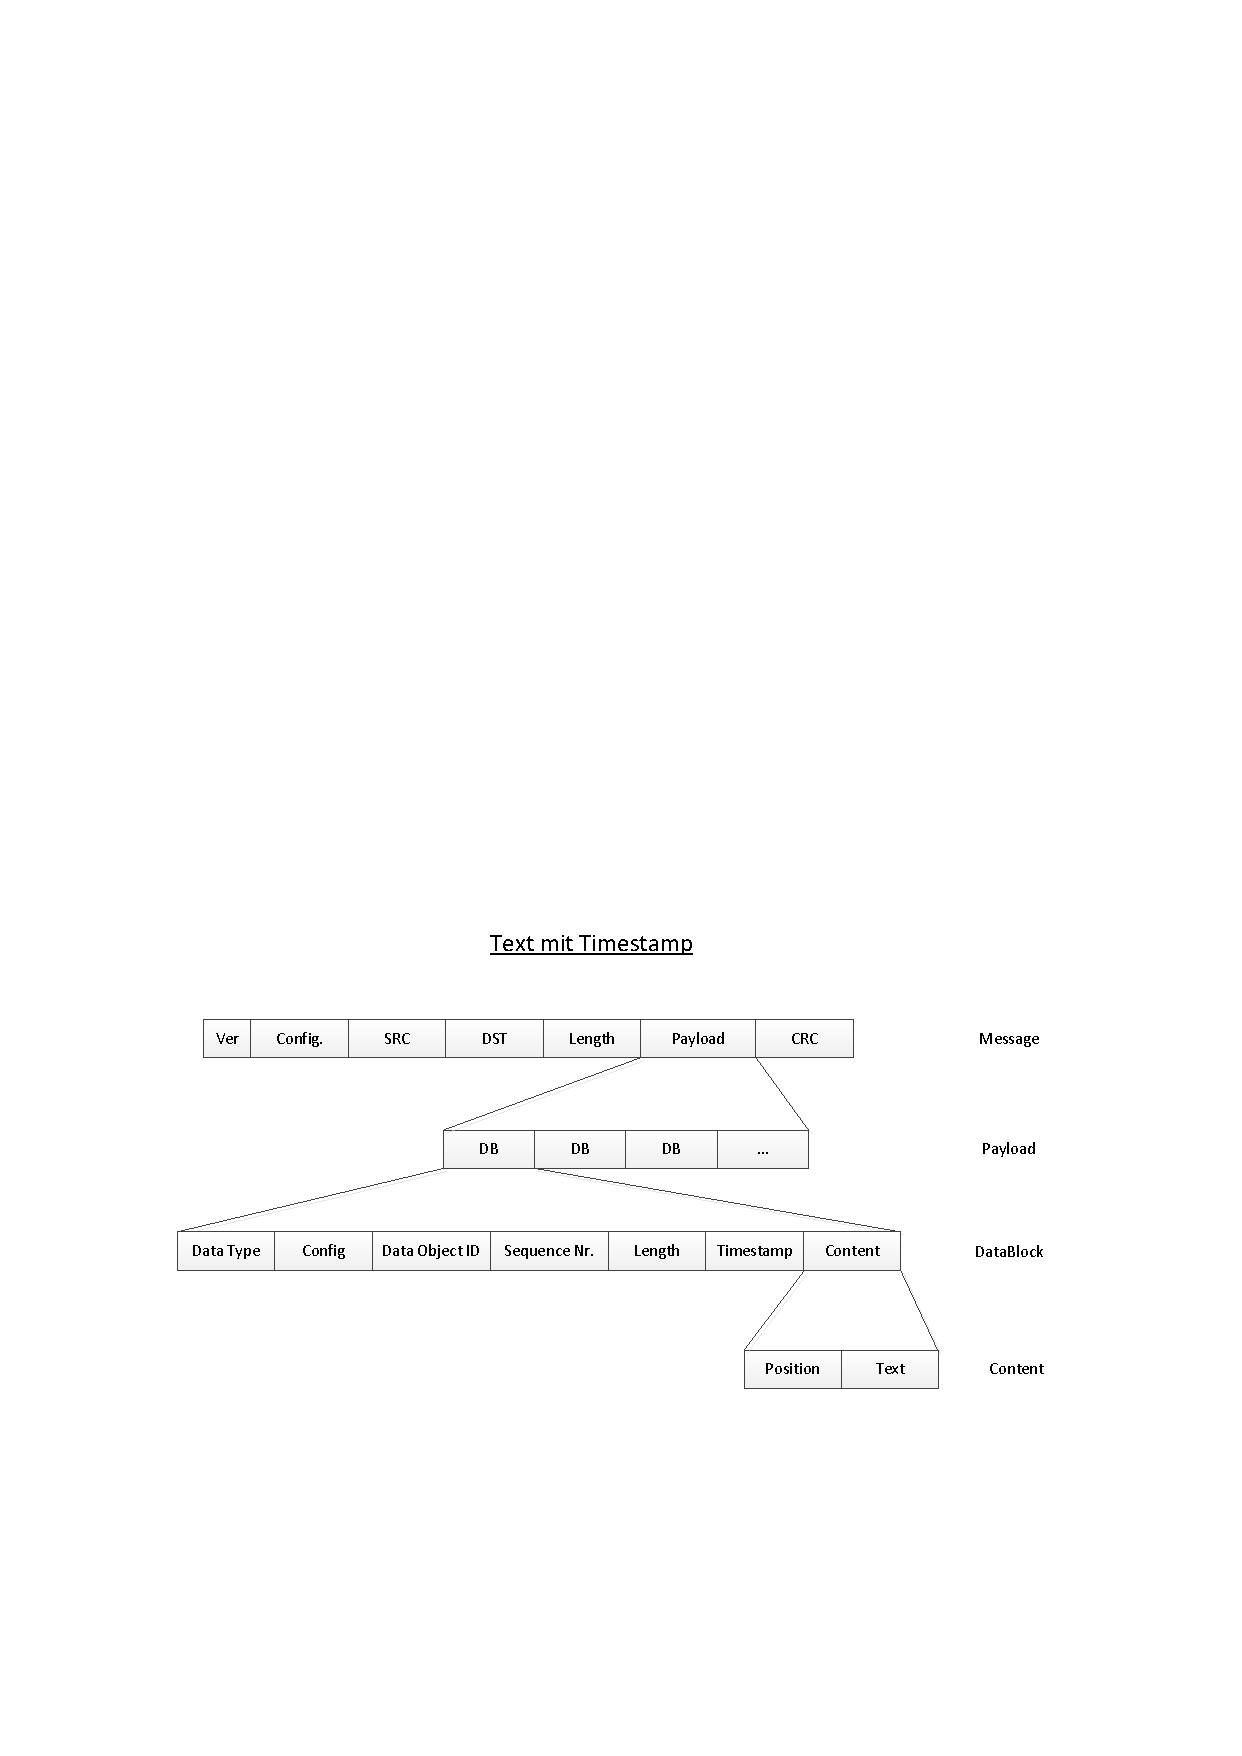
\includegraphics[width=\textwidth/2]{DatenaufschluesselungText.pdf}} 
  \caption{Übersicht der Datenaufschlüsselung}
  \label{fig:uebersichtdatenaufschluesselung}
\end{figure}

Durch den oben beschriebenen Aufbau wird eine flexible Handhabung
zahlreicher Datentypen ermöglicht. In Abbildung \ref{fig:beispielJPG} ist
dieser Vorgang anhand eines Bildes im Format JPEG dargestellt. Das Bild wird in mehrere
Datenblöcke zerlegt, welche die Bildinformationen (Content) beinhalten.
Diese wiederum bestehen aus einer Vielzahl an Pixeln.
Die Bildaten und der JPEG-Header bilden den Content. Ein Datenblock besteht
somit aus dem oben beschriebenen Content und dem dazugehörigen
Datenblockheader.

\begin{figure}[H]
	\centering
	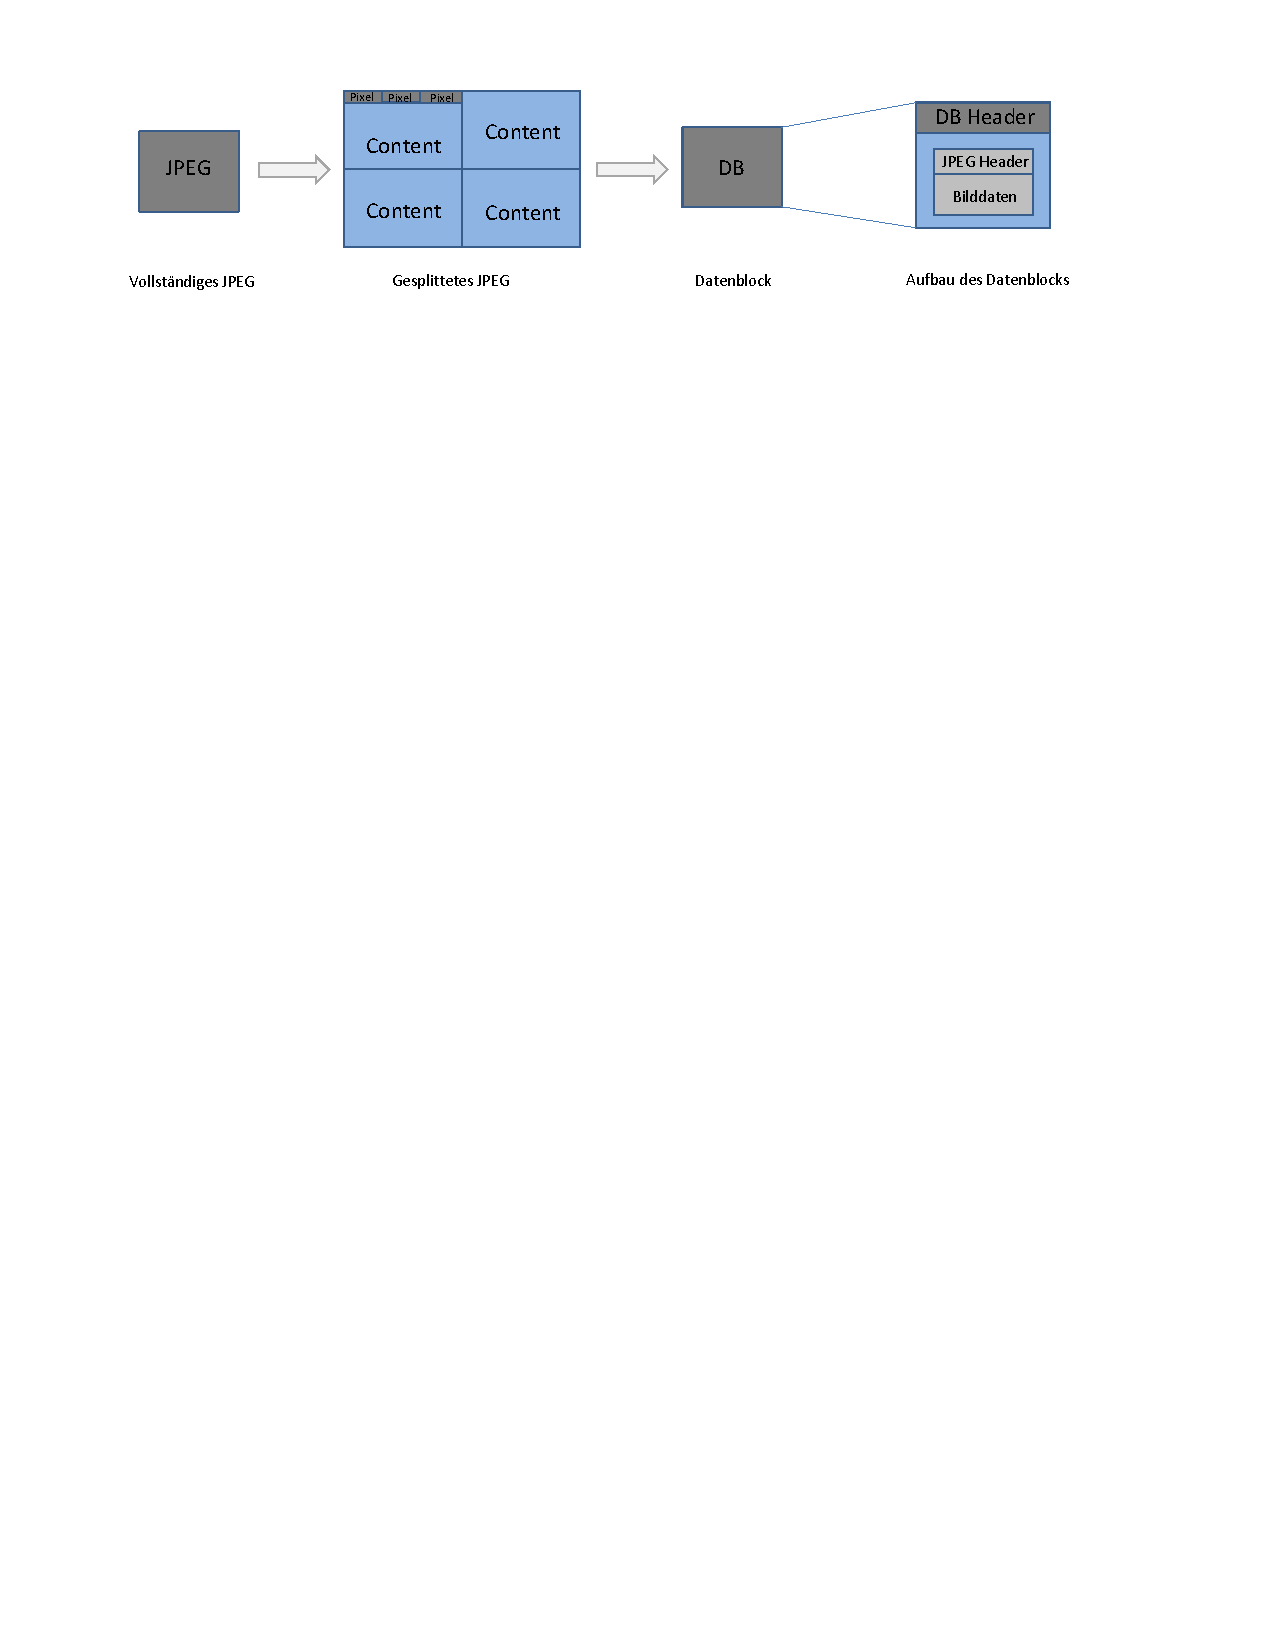
\includegraphics[width=\textwidth]{VerarbeitungJPEG-Bild.pdf}
	\caption{Verarbeitung eines JPEG-Bildes}
	\label{fig:beispielJPG}
\end{figure}

\textbf{Relevanz und Priorisierung}

Neben der Strukturierung und dem Aufbau der Nachricht selbst ist die
Wahl der Reihenfolge einzelner Datenblöcke sehr wichtig. Die Sortierung erfolgt
hierbei grundlegend in zwei Schritten, wie die Abbildung \ref{fig:priorisierungen}
zeigt.
Zunächst erfolgt eine Vorpriorisierung. Dabei werden relevante Bereiche
selektiert und mit einem Relevanzwert eingestuft. Die
Daten werden daraufhin in einzelne Blöcke zerlegt (siehe Abbildung
\ref{fig:priorisierungen} rechts) und erhalten abhängig ihrer Wichtigkeit einen
Prioritätswert. Danach erfolgt die Einsortierung der Datenblöcke unter
Berücksichtigung des Prioritätswertes in eine \gls{FIFO}.

\begin{figure}[H]
	\centering
	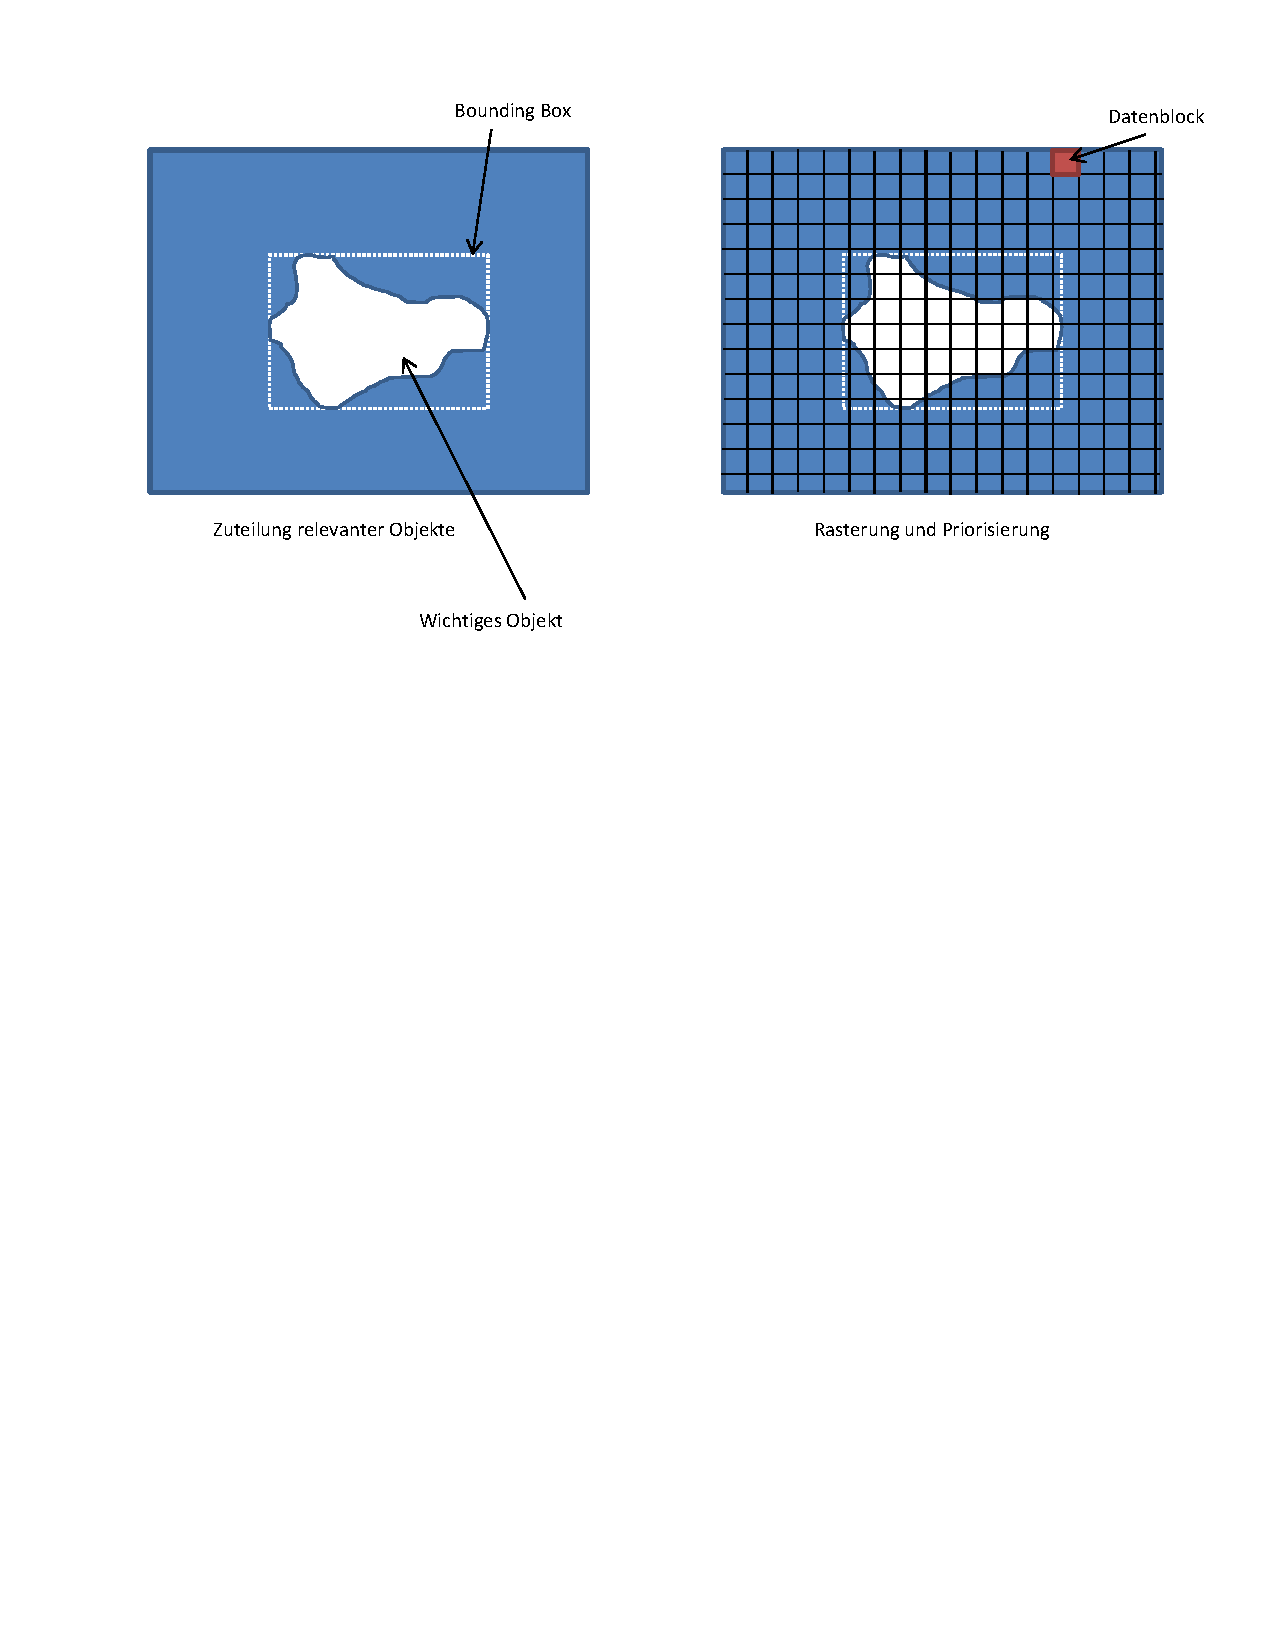
\includegraphics[width=\textwidth]{Priorisierung.pdf}
	\caption{Datenaufschlüsselung der Nachricht}
	\label{fig:priorisierungen}
\end{figure}
